

\tikzset{every picture/.style={line width=0.75pt}} %set default line width to 0.75pt        

\begin{tikzpicture}[x=0.75pt,y=0.75pt,yscale=-1,xscale=1]
%uncomment if require: \path (0,398); %set diagram left start at 0, and has height of 398

%Image [id:dp80183306204371] 
\draw (331.09,278) node  {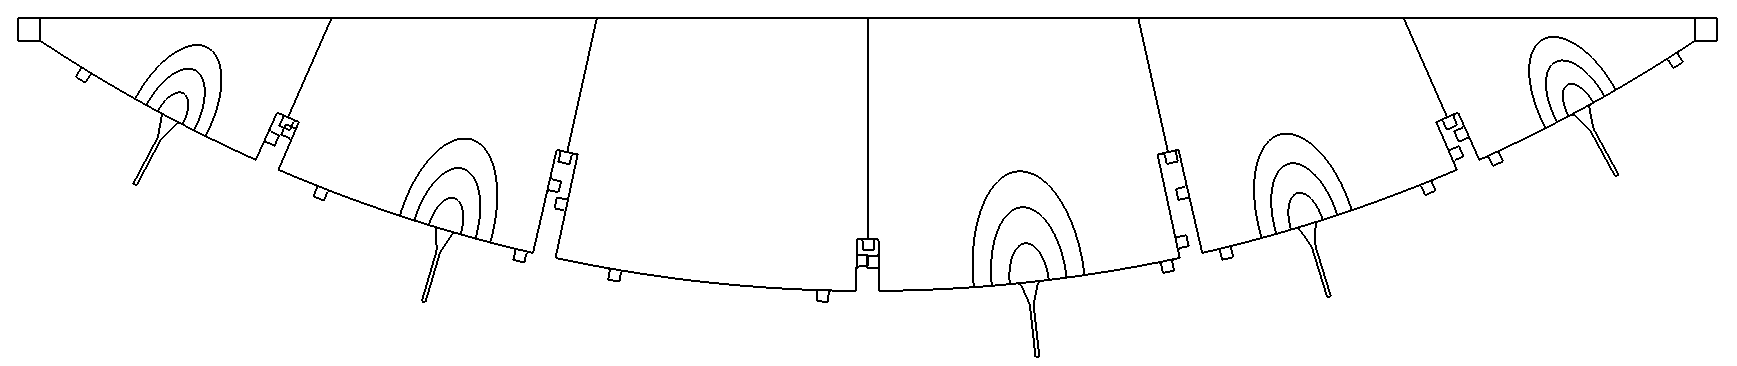
\includegraphics[width=473.38pt,height=100.5pt]{diagrams/placenta-geometry-diagrams/mesh_inverted-circle-slice-6-flat_normal-walls_septal-veins.png}};
%Shape: Polygon [id:ds599560967686122] 
\draw  [fill={rgb, 255:red, 155; green, 155; blue, 155 }  ,fill opacity=0.2 ] (436.42,180.33) -- (227,262.5) -- (215,262.5) -- (311.92,180.33) -- cycle ;
%Straight Lines [id:da3836552587833064] 
\draw [color={rgb, 255:red, 155; green, 155; blue, 155 }  ,draw opacity=1 ] [dash pattern={on 0.84pt off 2.51pt}]  (632.5,226.5) -- (632.5,345) ;
%Straight Lines [id:da8869549916108876] 
\draw [color={rgb, 255:red, 155; green, 155; blue, 155 }  ,draw opacity=1 ] [dash pattern={on 0.84pt off 2.51pt}]  (555,269) -- (555,345) ;
%Straight Lines [id:da08890647812691421] 
\draw [color={rgb, 255:red, 128; green, 128; blue, 128 }  ,draw opacity=1 ]   (558,345) -- (629.5,345) ;
\draw [shift={(632.5,345)}, rotate = 180] [fill={rgb, 255:red, 128; green, 128; blue, 128 }  ,fill opacity=1 ][line width=0.08]  [draw opacity=0] (7.14,-3.43) -- (0,0) -- (7.14,3.43) -- cycle    ;
\draw [shift={(555,345)}, rotate = 0] [fill={rgb, 255:red, 128; green, 128; blue, 128 }  ,fill opacity=1 ][line width=0.08]  [draw opacity=0] (7.14,-3.43) -- (0,0) -- (7.14,3.43) -- cycle    ;
%Straight Lines [id:da4569539433423251] 
\draw [color={rgb, 255:red, 155; green, 155; blue, 155 }  ,draw opacity=1 ] [dash pattern={on 0.84pt off 2.51pt}]  (545.5,273) -- (545.5,345) ;
%Straight Lines [id:da6425775020756577] 
\draw [color={rgb, 255:red, 155; green, 155; blue, 155 }  ,draw opacity=1 ] [dash pattern={on 0.84pt off 2.51pt}]  (453,303.5) -- (453,345) ;
%Straight Lines [id:da84971523704646] 
\draw [color={rgb, 255:red, 155; green, 155; blue, 155 }  ,draw opacity=1 ] [dash pattern={on 0.84pt off 2.51pt}]  (445.5,303.5) -- (445.5,344) ;
%Straight Lines [id:da4522901839526503] 
\draw [color={rgb, 255:red, 155; green, 155; blue, 155 }  ,draw opacity=1 ] [dash pattern={on 0.84pt off 2.51pt}]  (334.5,316) -- (334.5,344) ;
%Straight Lines [id:da886100326010987] 
\draw [color={rgb, 255:red, 128; green, 128; blue, 128 }  ,draw opacity=1 ]   (337.5,345) -- (442,345) ;
\draw [shift={(445,345)}, rotate = 180] [fill={rgb, 255:red, 128; green, 128; blue, 128 }  ,fill opacity=1 ][line width=0.08]  [draw opacity=0] (7.14,-3.43) -- (0,0) -- (7.14,3.43) -- cycle    ;
\draw [shift={(334.5,345)}, rotate = 0] [fill={rgb, 255:red, 128; green, 128; blue, 128 }  ,fill opacity=1 ][line width=0.08]  [draw opacity=0] (7.14,-3.43) -- (0,0) -- (7.14,3.43) -- cycle    ;
%Straight Lines [id:da2739622055496771] 
\draw [color={rgb, 255:red, 155; green, 155; blue, 155 }  ,draw opacity=1 ] [dash pattern={on 0.84pt off 2.51pt}]  (28.5,226.5) -- (28.5,345) ;
%Straight Lines [id:da8223757430798608] 
\draw [color={rgb, 255:red, 155; green, 155; blue, 155 }  ,draw opacity=1 ] [dash pattern={on 0.84pt off 2.51pt}]  (105.87,269.5) -- (105.87,345) ;
%Straight Lines [id:da9585020997428355] 
\draw [color={rgb, 255:red, 128; green, 128; blue, 128 }  ,draw opacity=1 ]   (102.87,345) -- (31.5,345) ;
\draw [shift={(28.5,345)}, rotate = 360] [fill={rgb, 255:red, 128; green, 128; blue, 128 }  ,fill opacity=1 ][line width=0.08]  [draw opacity=0] (7.14,-3.43) -- (0,0) -- (7.14,3.43) -- cycle    ;
\draw [shift={(105.87,345)}, rotate = 180] [fill={rgb, 255:red, 128; green, 128; blue, 128 }  ,fill opacity=1 ][line width=0.08]  [draw opacity=0] (7.14,-3.43) -- (0,0) -- (7.14,3.43) -- cycle    ;
%Straight Lines [id:da7396996741803523] 
\draw [color={rgb, 255:red, 155; green, 155; blue, 155 }  ,draw opacity=1 ] [dash pattern={on 0.84pt off 2.51pt}]  (115.35,273) -- (115.35,345) ;
%Straight Lines [id:da7690060794723255] 
\draw [color={rgb, 255:red, 155; green, 155; blue, 155 }  ,draw opacity=1 ] [dash pattern={on 0.84pt off 2.51pt}]  (207.7,303) -- (207.7,345) ;
%Straight Lines [id:da1750801006916194] 
\draw [color={rgb, 255:red, 155; green, 155; blue, 155 }  ,draw opacity=1 ] [dash pattern={on 0.84pt off 2.51pt}]  (215.19,305) -- (215.19,344) ;
%Straight Lines [id:da36519166335869224] 
\draw [color={rgb, 255:red, 155; green, 155; blue, 155 }  ,draw opacity=1 ] [dash pattern={on 0.84pt off 2.51pt}]  (326,316.5) -- (326,344) ;
%Straight Lines [id:da5227117484890365] 
\draw [color={rgb, 255:red, 128; green, 128; blue, 128 }  ,draw opacity=1 ]   (323,345) -- (218.69,345) ;
\draw [shift={(215.69,345)}, rotate = 360] [fill={rgb, 255:red, 128; green, 128; blue, 128 }  ,fill opacity=1 ][line width=0.08]  [draw opacity=0] (7.14,-3.43) -- (0,0) -- (7.14,3.43) -- cycle    ;
\draw [shift={(326,345)}, rotate = 180] [fill={rgb, 255:red, 128; green, 128; blue, 128 }  ,fill opacity=1 ][line width=0.08]  [draw opacity=0] (7.14,-3.43) -- (0,0) -- (7.14,3.43) -- cycle    ;
%Straight Lines [id:da9869684148666715] 
\draw [color={rgb, 255:red, 128; green, 128; blue, 128 }  ,draw opacity=1 ]   (204.2,345) -- (118.35,345) ;
\draw [shift={(115.35,345)}, rotate = 360] [fill={rgb, 255:red, 128; green, 128; blue, 128 }  ,fill opacity=1 ][line width=0.08]  [draw opacity=0] (7.14,-3.43) -- (0,0) -- (7.14,3.43) -- cycle    ;
\draw [shift={(207.2,345)}, rotate = 180] [fill={rgb, 255:red, 128; green, 128; blue, 128 }  ,fill opacity=1 ][line width=0.08]  [draw opacity=0] (7.14,-3.43) -- (0,0) -- (7.14,3.43) -- cycle    ;
%Shape: Rectangle [id:dp7784307888916284] 
\draw   (379,303.5) -- (396.5,303.5) -- (396.5,341.5) -- (379,341.5) -- cycle ;
%Shape: Rectangle [id:dp7413532166529391] 
\draw   (18,215.27) -- (35.5,215.27) -- (35.5,228.77) -- (18,228.77) -- cycle ;
%Shape: Rectangle [id:dp1083356594712217] 
\draw   (305.17,310.67) -- (322.67,310.67) -- (322.67,326.17) -- (305.17,326.17) -- cycle ;
%Shape: Polygon [id:ds13903772067200593] 
\draw  [fill={rgb, 255:red, 155; green, 155; blue, 155 }  ,fill opacity=0.2 ] (635,183) -- (396.5,303.5) -- (379,303.5) -- (463.75,183) -- cycle ;
%Shape: Polygon [id:ds6960752336656928] 
\draw  [fill={rgb, 255:red, 155; green, 155; blue, 155 }  ,fill opacity=0.2 ] (139.25,187.75) -- (35.5,215.27) -- (18,215.27) -- (14.75,187.75) -- cycle ;
%Shape: Polygon [id:ds16525050807756858] 
\draw  [fill={rgb, 255:red, 155; green, 155; blue, 155 }  ,fill opacity=0.2 ] (436.42,180.33) -- (322.67,310.67) -- (305.17,310.67) -- (311.92,180.33) -- cycle ;
%Shape: Rectangle [id:dp6070840373099016] 
\draw  [color={rgb, 255:red, 208; green, 2; blue, 27 }  ,draw opacity=1 ][fill={rgb, 255:red, 255; green, 255; blue, 255 }  ,fill opacity=1 ][line width=2.25] [blur shadow={shadow xshift=0pt,shadow yshift=0pt, shadow blur radius=1.5pt, shadow blur steps=4 ,shadow opacity=100}] (463.75,22.5) -- (635,22.5) -- (635,183) -- (463.75,183) -- cycle ;
%Image [id:dp7341682961381069] 
\draw (523.25,97.77) node  {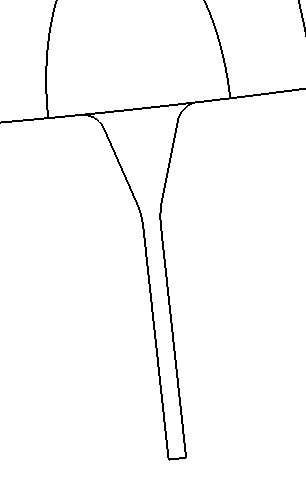
\includegraphics[width=54.75pt,height=89.28pt]{diagrams/placenta-geometry-diagrams/mesh_inverted-circle-slice-6-flat_normal-walls-septal-veins_artery.png}};
%Straight Lines [id:da2560686325124286] 
\draw [color={rgb, 255:red, 155; green, 155; blue, 155 }  ,draw opacity=1 ] [dash pattern={on 0.84pt off 2.51pt}]  (532.75,63) -- (575,57.75) ;
%Straight Lines [id:da862538474933769] 
\draw [color={rgb, 255:red, 155; green, 155; blue, 155 }  ,draw opacity=1 ] [dash pattern={on 0.84pt off 2.51pt}]  (531.25,150.75) -- (585.75,143.5) ;
%Straight Lines [id:da07631904575656989] 
\draw [color={rgb, 255:red, 128; green, 128; blue, 128 }  ,draw opacity=1 ]   (585.36,137.02) -- (575.64,61.98) ;
\draw [shift={(575.25,59)}, rotate = 82.61] [fill={rgb, 255:red, 128; green, 128; blue, 128 }  ,fill opacity=1 ][line width=0.08]  [draw opacity=0] (7.14,-3.43) -- (0,0) -- (7.14,3.43) -- cycle    ;
\draw [shift={(585.75,140)}, rotate = 262.61] [fill={rgb, 255:red, 128; green, 128; blue, 128 }  ,fill opacity=1 ][line width=0.08]  [draw opacity=0] (7.14,-3.43) -- (0,0) -- (7.14,3.43) -- cycle    ;
%Straight Lines [id:da9334742103638392] 
\draw [color={rgb, 255:red, 128; green, 128; blue, 128 }  ,draw opacity=1 ]   (526.19,150.18) -- (492.5,129.5) ;
\draw [shift={(528.75,151.75)}, rotate = 211.54] [fill={rgb, 255:red, 128; green, 128; blue, 128 }  ,fill opacity=1 ][line width=0.08]  [draw opacity=0] (6.25,-3) -- (0,0) -- (6.25,3) -- cycle    ;
%Straight Lines [id:da644000948100526] 
\draw [color={rgb, 255:red, 128; green, 128; blue, 128 }  ,draw opacity=1 ]   (535.18,86.02) -- (533.07,65.98) ;
\draw [shift={(532.75,63)}, rotate = 83.96] [fill={rgb, 255:red, 128; green, 128; blue, 128 }  ,fill opacity=1 ][line width=0.08]  [draw opacity=0] (5.36,-2.57) -- (0,0) -- (5.36,2.57) -- cycle    ;
\draw [shift={(535.5,89)}, rotate = 263.96] [fill={rgb, 255:red, 128; green, 128; blue, 128 }  ,fill opacity=1 ][line width=0.08]  [draw opacity=0] (5.36,-2.57) -- (0,0) -- (5.36,2.57) -- cycle    ;
%Straight Lines [id:da058958443439840025] 
\draw [color={rgb, 255:red, 155; green, 155; blue, 155 }  ,draw opacity=1 ] [dash pattern={on 0.84pt off 2.51pt}]  (526,89.75) -- (535.5,89) ;
%Straight Lines [id:da635774139796158] 
\draw [color={rgb, 255:red, 128; green, 128; blue, 128 }  ,draw opacity=1 ]   (528.02,57.33) -- (509.23,59.42) ;
\draw [shift={(506.25,59.75)}, rotate = 353.66] [fill={rgb, 255:red, 128; green, 128; blue, 128 }  ,fill opacity=1 ][line width=0.08]  [draw opacity=0] (5.36,-2.57) -- (0,0) -- (5.36,2.57) -- cycle    ;
\draw [shift={(531,57)}, rotate = 173.66] [fill={rgb, 255:red, 128; green, 128; blue, 128 }  ,fill opacity=1 ][line width=0.08]  [draw opacity=0] (5.36,-2.57) -- (0,0) -- (5.36,2.57) -- cycle    ;
%Shape: Rectangle [id:dp12087627646558885] 
\draw  [color={rgb, 255:red, 74; green, 144; blue, 226 }  ,draw opacity=1 ][fill={rgb, 255:red, 255; green, 255; blue, 255 }  ,fill opacity=1 ][line width=2.25] [blur shadow={shadow xshift=0pt,shadow yshift=0pt, shadow blur radius=1.5pt, shadow blur steps=4 ,shadow opacity=100}] (311.92,51.5) -- (436.42,51.5) -- (436.42,180.33) -- (311.92,180.33) -- cycle ;
%Image [id:dp11084122971065935] 
\draw (362.92,87.84) node  {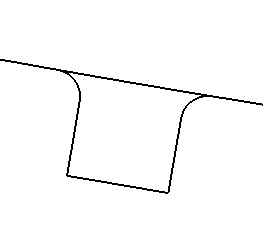
\includegraphics[width=56.25pt,height=51.76pt]{diagrams/placenta-geometry-diagrams/mesh_inverted-circle-slice-6-flat_normal-walls-septal-veins_vein.png}};
%Straight Lines [id:da4260411781736031] 
\draw [color={rgb, 255:red, 128; green, 128; blue, 128 }  ,draw opacity=1 ]   (371.2,114.18) -- (344.25,110.16) ;
\draw [shift={(341.28,109.72)}, rotate = 8.49] [fill={rgb, 255:red, 128; green, 128; blue, 128 }  ,fill opacity=1 ][line width=0.08]  [draw opacity=0] (5.36,-2.57) -- (0,0) -- (5.36,2.57) -- cycle    ;
\draw [shift={(374.17,114.63)}, rotate = 188.49] [fill={rgb, 255:red, 128; green, 128; blue, 128 }  ,fill opacity=1 ][line width=0.08]  [draw opacity=0] (5.36,-2.57) -- (0,0) -- (5.36,2.57) -- cycle    ;
%Straight Lines [id:da13622705064859697] 
\draw [color={rgb, 255:red, 128; green, 128; blue, 128 }  ,draw opacity=1 ]   (383.91,85.29) -- (380.42,105.63) ;
\draw [shift={(379.92,108.58)}, rotate = 279.73] [fill={rgb, 255:red, 128; green, 128; blue, 128 }  ,fill opacity=1 ][line width=0.08]  [draw opacity=0] (5.36,-2.57) -- (0,0) -- (5.36,2.57) -- cycle    ;
\draw [shift={(384.42,82.33)}, rotate = 99.73] [fill={rgb, 255:red, 128; green, 128; blue, 128 }  ,fill opacity=1 ][line width=0.08]  [draw opacity=0] (5.36,-2.57) -- (0,0) -- (5.36,2.57) -- cycle    ;
%Shape: Rectangle [id:dp043044360722185315] 
\draw  [color={rgb, 255:red, 74; green, 144; blue, 226 }  ,draw opacity=1 ][fill={rgb, 255:red, 255; green, 255; blue, 255 }  ,fill opacity=1 ][line width=2.25] [blur shadow={shadow xshift=0pt,shadow yshift=0pt, shadow blur radius=1.5pt, shadow blur steps=4 ,shadow opacity=100}] (14.75,110.5) -- (139.25,110.5) -- (139.25,187.75) -- (14.75,187.75) -- cycle ;
%Image [id:dp43909768466905374] 
\draw (88.25,149.86) node [xscale=-1] {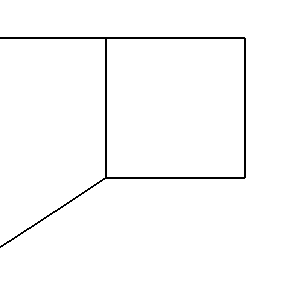
\includegraphics[width=52.5pt,height=53.05pt]{diagrams/placenta-geometry-diagrams/mesh_inverted-circle-slice-6-flat_normal-walls-septal-veins_marginal-sinus.png}};
%Straight Lines [id:da33088686310200743] 
\draw [color={rgb, 255:red, 128; green, 128; blue, 128 }  ,draw opacity=1 ]   (94,161.75) -- (66.75,161.75) ;
\draw [shift={(63.75,161.75)}, rotate = 360] [fill={rgb, 255:red, 128; green, 128; blue, 128 }  ,fill opacity=1 ][line width=0.08]  [draw opacity=0] (5.36,-2.57) -- (0,0) -- (5.36,2.57) -- cycle    ;
\draw [shift={(97,161.75)}, rotate = 180] [fill={rgb, 255:red, 128; green, 128; blue, 128 }  ,fill opacity=1 ][line width=0.08]  [draw opacity=0] (5.36,-2.57) -- (0,0) -- (5.36,2.57) -- cycle    ;
%Straight Lines [id:da3164833140775334] 
\draw [color={rgb, 255:red, 128; green, 128; blue, 128 }  ,draw opacity=1 ]   (57.75,125.5) -- (57.75,152.75) ;
\draw [shift={(57.75,155.75)}, rotate = 270] [fill={rgb, 255:red, 128; green, 128; blue, 128 }  ,fill opacity=1 ][line width=0.08]  [draw opacity=0] (5.36,-2.57) -- (0,0) -- (5.36,2.57) -- cycle    ;
\draw [shift={(57.75,122.5)}, rotate = 90] [fill={rgb, 255:red, 128; green, 128; blue, 128 }  ,fill opacity=1 ][line width=0.08]  [draw opacity=0] (5.36,-2.57) -- (0,0) -- (5.36,2.57) -- cycle    ;
%Shape: Rectangle [id:dp3214087399382912] 
\draw  [color={rgb, 255:red, 65; green, 117; blue, 5 }  ,draw opacity=1 ][dash pattern={on 2.53pt off 3.02pt}][line width=2.25]  (264.5,303) -- (281.5,303) -- (281.5,320) -- (264.5,320) -- cycle ;
%Shape: Axis 2D [id:dp5493960903283415] 
\draw  (10.68,368.48) -- (43.48,368.48)(13.96,338.96) -- (13.96,371.76) (36.48,363.48) -- (43.48,368.48) -- (36.48,373.48) (8.96,345.96) -- (13.96,338.96) -- (18.96,345.96)  ;

%Straight Lines [id:da8673543563072263] 
\draw [color={rgb, 255:red, 65; green, 117; blue, 5 }  ,draw opacity=1 ]   (244.5,173) -- (273.01,293.58) ;
\draw [shift={(273.7,296.5)}, rotate = 256.7] [fill={rgb, 255:red, 65; green, 117; blue, 5 }  ,fill opacity=1 ][line width=0.08]  [draw opacity=0] (8.93,-4.29) -- (0,0) -- (8.93,4.29) -- cycle    ;
%Straight Lines [id:da15777572686334396] 
\draw [color={rgb, 255:red, 128; green, 128; blue, 128 }  ,draw opacity=1 ]   (456.5,345) -- (542.5,345) ;
\draw [shift={(545.5,345)}, rotate = 180] [fill={rgb, 255:red, 128; green, 128; blue, 128 }  ,fill opacity=1 ][line width=0.08]  [draw opacity=0] (7.14,-3.43) -- (0,0) -- (7.14,3.43) -- cycle    ;
\draw [shift={(453.5,345)}, rotate = 0] [fill={rgb, 255:red, 128; green, 128; blue, 128 }  ,fill opacity=1 ][line width=0.08]  [draw opacity=0] (7.14,-3.43) -- (0,0) -- (7.14,3.43) -- cycle    ;
%Straight Lines [id:da20967786638483576] 
\draw [color={rgb, 255:red, 128; green, 128; blue, 128 }  ,draw opacity=1 ]   (126.53,260.24) -- (121.97,270.51) ;
\draw [shift={(120.75,273.25)}, rotate = 293.96] [fill={rgb, 255:red, 128; green, 128; blue, 128 }  ,fill opacity=1 ][line width=0.08]  [draw opacity=0] (3.57,-1.72) -- (0,0) -- (3.57,1.72) -- cycle    ;
\draw [shift={(127.75,257.5)}, rotate = 113.96] [fill={rgb, 255:red, 128; green, 128; blue, 128 }  ,fill opacity=1 ][line width=0.08]  [draw opacity=0] (3.57,-1.72) -- (0,0) -- (3.57,1.72) -- cycle    ;
%Straight Lines [id:da999991789814658] 
\draw [color={rgb, 255:red, 128; green, 128; blue, 128 }  ,draw opacity=1 ]   (228.14,272.19) -- (222.1,301.15) ;
\draw [shift={(221.49,304.09)}, rotate = 281.77] [fill={rgb, 255:red, 128; green, 128; blue, 128 }  ,fill opacity=1 ][line width=0.08]  [draw opacity=0] (3.57,-1.72) -- (0,0) -- (3.57,1.72) -- cycle    ;
\draw [shift={(228.75,269.25)}, rotate = 101.77] [fill={rgb, 255:red, 128; green, 128; blue, 128 }  ,fill opacity=1 ][line width=0.08]  [draw opacity=0] (3.57,-1.72) -- (0,0) -- (3.57,1.72) -- cycle    ;
%Shape: Rectangle [id:dp842610769802747] 
\draw   (215,262.5) -- (227,262.5) -- (227,272.5) -- (215,272.5) -- cycle ;
%Shape: Rectangle [id:dp34481258515956204] 
\draw  [color={rgb, 255:red, 65; green, 117; blue, 5 }  ,draw opacity=1 ][dash pattern={on 2.53pt off 3.02pt}][line width=2.25]  (94,260.5) -- (106,260.5) -- (106,272) -- (94,272) -- cycle ;
%Straight Lines [id:da484653672836302] 
\draw [color={rgb, 255:red, 65; green, 117; blue, 5 }  ,draw opacity=1 ]   (187.5,196.5) -- (107.93,254.24) ;
\draw [shift={(105.5,256)}, rotate = 324.03] [fill={rgb, 255:red, 65; green, 117; blue, 5 }  ,fill opacity=1 ][line width=0.08]  [draw opacity=0] (8.93,-4.29) -- (0,0) -- (8.93,4.29) -- cycle    ;

% Text Node
\draw (67.18,348.4) node [anchor=north] [inner sep=0.75pt]  [font=\footnotesize,color={rgb, 255:red, 128; green, 128; blue, 128 }  ,opacity=1 ]  {$28.65\ \text{mm}$};
% Text Node
\draw (161.28,348.4) node [anchor=north] [inner sep=0.75pt]  [font=\footnotesize,color={rgb, 255:red, 128; green, 128; blue, 128 }  ,opacity=1 ]  {$33.85\ \text{mm}$};
% Text Node
\draw (270.84,348.4) node [anchor=north] [inner sep=0.75pt]  [font=\footnotesize,color={rgb, 255:red, 128; green, 128; blue, 128 }  ,opacity=1 ]  {$40\ \text{mm}$};
% Text Node
\draw (389.75,348.4) node [anchor=north] [inner sep=0.75pt]  [font=\footnotesize,color={rgb, 255:red, 128; green, 128; blue, 128 }  ,opacity=1 ]  {$40\ \text{mm}$};
% Text Node
\draw (499.5,348.4) node [anchor=north] [inner sep=0.75pt]  [font=\footnotesize,color={rgb, 255:red, 128; green, 128; blue, 128 }  ,opacity=1 ]  {$33.85\ \text{mm}$};
% Text Node
\draw (593.75,348.4) node [anchor=north] [inner sep=0.75pt]  [font=\footnotesize,color={rgb, 255:red, 128; green, 128; blue, 128 }  ,opacity=1 ]  {$28.65\ \text{mm}$};
% Text Node
\draw (582.5,99.5) node [anchor=west] [inner sep=0.75pt]  [font=\footnotesize,color={rgb, 255:red, 128; green, 128; blue, 128 }  ,opacity=1 ]  {$10\ \text{mm}$};
% Text Node
\draw (512.64,126.72) node [anchor=south east] [inner sep=0.75pt]  [font=\scriptsize,color={rgb, 255:red, 128; green, 128; blue, 128 }  ,opacity=1 ]  {$0.5\ \text{mm}$};
% Text Node
\draw (536.13,76) node [anchor=west] [inner sep=0.75pt]  [font=\scriptsize,color={rgb, 255:red, 128; green, 128; blue, 128 }  ,opacity=1 ]  {$3\ \text{mm}$};
% Text Node
\draw (518.63,54.98) node [anchor=south] [inner sep=0.75pt]  [font=\scriptsize,color={rgb, 255:red, 128; green, 128; blue, 128 }  ,opacity=1 ]  {$2.4\ \text{mm}$};
% Text Node
\draw (80.38,165.15) node [anchor=north] [inner sep=0.75pt]  [font=\scriptsize,color={rgb, 255:red, 128; green, 128; blue, 128 }  ,opacity=1 ]  {$3\ \text{mm}$};
% Text Node
\draw (55.75,139.13) node [anchor=east] [inner sep=0.75pt]  [font=\scriptsize,color={rgb, 255:red, 128; green, 128; blue, 128 }  ,opacity=1 ]  {$3\ \text{mm}$};
% Text Node
\draw (357.22,115.53) node [anchor=north] [inner sep=0.75pt]  [font=\scriptsize,color={rgb, 255:red, 128; green, 128; blue, 128 }  ,opacity=1 ,rotate=-8.49]  {$1.5\ \text{mm}$};
% Text Node
\draw (384.14,95.75) node [anchor=west] [inner sep=0.75pt]  [font=\scriptsize,color={rgb, 255:red, 128; green, 128; blue, 128 }  ,opacity=1 ,rotate=-8.49]  {$1.5\ \text{mm}$};
% Text Node
\draw (46.86,365) node [anchor=west] [inner sep=0.75pt]  [font=\footnotesize]  {$x$};
% Text Node
\draw (15,332.55) node [anchor=south] [inner sep=0.75pt]  [font=\footnotesize]  {$y$};
% Text Node
\draw (373.4,139.41) node [anchor=north] [inner sep=0.75pt]  [font=\small] [align=left] {\textcolor[rgb]{0.29,0.56,0.89}{basal plate and}\\\textcolor[rgb]{0.29,0.56,0.89}{septal wall veins}};
% Text Node
\draw (545.5,174.4) node [anchor=south] [inner sep=0.75pt]  [font=\small,color={rgb, 255:red, 208; green, 2; blue, 27 }  ,opacity=1 ] [align=left] {spiral artery};
% Text Node
\draw (126.02,266.74) node [anchor=west] [inner sep=0.75pt]  [font=\tiny,color={rgb, 255:red, 128; green, 128; blue, 128 }  ,opacity=1 ,rotate=-23.4]  {$6.90\ \text{mm}$};
% Text Node
\draw (227.07,287.11) node [anchor=west] [inner sep=0.75pt]  [font=\tiny,color={rgb, 255:red, 128; green, 128; blue, 128 }  ,opacity=1 ,rotate=-12.55]  {$14.07\ \text{mm}$};
% Text Node
\draw (202.23,156.01) node [anchor=north west][inner sep=0.75pt]  [font=\small,color={rgb, 255:red, 65; green, 117; blue, 5 }  ,opacity=1 ] [align=left] {omitted artery};
% Text Node
\draw (153.73,179.51) node [anchor=north west][inner sep=0.75pt]  [font=\small,color={rgb, 255:red, 65; green, 117; blue, 5 }  ,opacity=1 ] [align=left] {omitted vein};


\end{tikzpicture}
